\chapter{Performance and optimization}
In this chapter, we will justify some choices that we made in the code that increase efficiency.
In the process, we will show and analyze the output of some optimization tools we used in order to test the performance of this library, as well as some of the aforementioned choices.

\section{Compiler flags} \label{opt-flags}
When calling the \verb|g++| complier from the \verb|Makefile|, we used the following optimization flags, which instruct the compiler to maximize the code efficiency:
\begin{verbatim}
-march=native -O3 -msse2 -funroll-loops -ftree-vectorize
\end{verbatim}
In order to test their effects, we ran the \verb|maintest_nnws.cpp| test file (which has the standard combination of the \verb|HierarchyNNW<HypersFixedNNW>| plus the \verb|DirichletMixture| class) using $n=10$ 5-dimensional data points and a 7-point grid for the density evaluation, with and without the above flags, while timing both the algorithm execution and the density estimate with the help of the \verb|chrono| library.
We use $n=10$ because in such a high dimension, even computation times on a handful of points become extremely large and can lead to overflow.
The obtained average times in shakes (a metric unit of time equal to 10 nanoseconds) were as follows:
\begin{center}
	\begin{tabular}{r|r|r|r}
	              	& \verb|run()| & \verb|eval_density()| & total \\ \hline
		without flags & 521762512 & 182770170 & 704532682 \\
		with flags    &  39615848 &  10353269 &  49969117 \\
		speedup       &       13x &       17x &       14x
	\end{tabular}
\end{center}
As one can see, the speedup resulting from the addition of these flags is hugely noticeable.


\section{In the \texttt{Algorithm} class}
One might note that the cluster cardinalities need not be part of the state, since they can be computed at any time from the allocations.
Despite that, we store the \verb|cardinalities| of the current iteration in a vector, which is first filled when the initial clusters are being built in the \verb|initialize()| function, then updated after the repositioning of each datum in \verb|sample_allocations()|.
This is because their explicit computation is needed in \verb|sample_allocations()| in order to be able to compute the masses of the current clusters.
The alternative is rebuilding the vector at each call of \verb|sample_allocations()|, which is $O(n)$; this is the same cost as the worst-case scenario of storing them externally, which can potentially happen in case 2.
In particular, if the first cluster is a singleton and the current datum moves from it to any other cluster, the whole vector must be shifted to the left by 1.
Therefore, the external storage is clearly a better choice. \\[8pt]
A second point involves the usage of sparse Eigen matrices instead of dense ones in \verb|cluster_estimate()|.
It is mandatory to store the dissimilarity matrix for each of the $K$ iterations must be stored, so that the Frobenius norm of its difference with the mean dissimilarity can be computed.
These matrices add up to a total of $K n^2$ entries.
When the data size starts being moderately large, the memory usage becomes huge if using regular dense matrices.
On the contrary, the \verb|Eigen::SparseMatrix| class stores data points as a double vector of position and value, therefore greatly reducing the number of entries in the object, from $n^2$ to $2n$.
The dissimilarity matrices are indeed sparse objects, since their upper triangular part is never filled, and several of the entries in the lower triangular part may be zero as well.
In order to fill this type of matrix, a vector \verb|triplets_list| of \verb|Eigen::Triplet| objects must be used which stores each entry's position and value; the \verb|setFromTriplets()| method of the matrix is then used by passing \verb|triplets_list| as argument.
In order not to waste time reallocating massive amounts of data, a \verb|triplets_list.reserve()| call, and an estimate for the number of entries, are thus desirable.
Suppose that the $n$ data points are evenly distributed into $k$ clusters.
In such a case, the number of nonzero entries for the corresponding dissimilarity matrix (without the upper triangular part) is
$$ k \left(\binom{n/k}{2} - n\right) = \frac{n^2}{2k} -\frac{n}{2} - nk,$$
whilst the number for unbalanced clusters is slightly higher.
Therefore, $\frac{n^2}{4}$ is a good estimate for the number of entries.
This number is very close to the true amount if the number of clusters is small (e.g. $k=2,3,4$), which it often is. (Note that one could theoretically compute the exact number of nonzero entries of the dissimilarity matrix, but this would require additional computational costs which is not warranted for the size of a single vector.)
This relatively large amount of reserved space does not significantly impact the overall memory usage, since the \verb|triplets_list| vector is destroyed after each dissimilarity matrix is computed. \\
The usage of sparse matrices instead of dense ones does not hinder computational time either, since the Eigen library also heavily optimizes computations with sparse objects.
Nevertheless, an efficiency test was performed, this time using the Python interface, on the already implemented Python tests 1-6 (see section \ref{chap-py-test} for full details) with 500 algorithm iterations and 100 burn-in ones, using sparse matrices first and then the same operations but with dense matrices.
The results were as follows, again in shakes:
\begin{center}
	\begin{tabular}{c|c|c}
       &      sparse    &      dense     \\ \hline
test 1 & 4.51696840e+07 & 4.15315598e+07 \\
test 2 & 1.18633301e+09 & 9.17060859e+08 \\
test 3 & 2.91540577e+07 & 3.00693867e+07 \\
test 4 & 1.27339513e+08 & 1.22764857e+08 \\
test 5 & 1.50049441e+08 & 1.37240555e+08 \\
test 6 & 1.28818714e+08 & 1.16328396e+08
	\end{tabular}
\end{center}
As one can see, the performance is on average nearly identical for both types of implementation, with a difference of only less than 10\% for the multivariate tests 5 and 6 in favor of the dense case. \\[8pt]
Finally, one more possible improvement for the current implementation is using a completely different approach of storing the data, e.g. with an \verb|std::map| in which each entry is a cluster that holds objects representing the data points themselves, instead of just storing the allocations labels.
This may be a way to erase and add clusters more efficiently.
Testing this assumption would be very difficult, since it would require implementing all data structures from scratch; nonetheless we think that using vectorial structures is more efficient for everything else, and therefore the correct choice.


\section{In the \texttt{Hierarchy} classes}
It was mentioned earlier that our custom implementation of the data likelihood in \verb|HierarchyNNW| was more efficient than the one provided by the Stan library.
The difference becomes more and more relevant as the data dimension increases, since there are matricial operations involved.
We ran some tests, again in \verb|maintest_nnws.cpp|, to quantify the time saved, using the same 5-dimensional dataset and grid as before.
Note that the \verb|like()| function is used not only in density estimation, but also in the allocation sampling phase of the algorithm, thus it affects \verb|run()| as well.
We include the average results:
\begin{center}
	\begin{tabular}{r|r|r|r}
		& \verb|run()| & \verb|eval_density()| & total \\ \hline
		   Stan & 47700683 & 14317337 & 62018020 \\
		 custom & 39615848 & 10353269 & 49969117 \\
		speedup &    1.20x &    1.38x &    1.25x
	\end{tabular}
\end{center}


\section{Profiling analysis}
\verb|callgrind| is a command-line profiling tool that observes the running of the executable it is given as argument and records the call history among all functions that were called in it.
The output is then saved in a \verb|callgrind.out| file, which can be read with the use of the KCacheGrind GUI.
The following two commands were run, each on the C++ main test file for both the univariate case (with \verb|HierarchyNNIG<HypersFixedNNIG>|) and the multivariate case (with \verb|HierarchyNNW<HypersFixedNNW>|):
\begin{verbatim}
valgrind --tool=callgrind ./maintest_uni csv/data_uni.csv neal2 memory
valgrind --tool=callgrind ./maintest_multi csv/data_multi.csv neal2 memory
\end{verbatim}
\begin{figure}[h]
	%\centering
	\hspace{-50pt}
	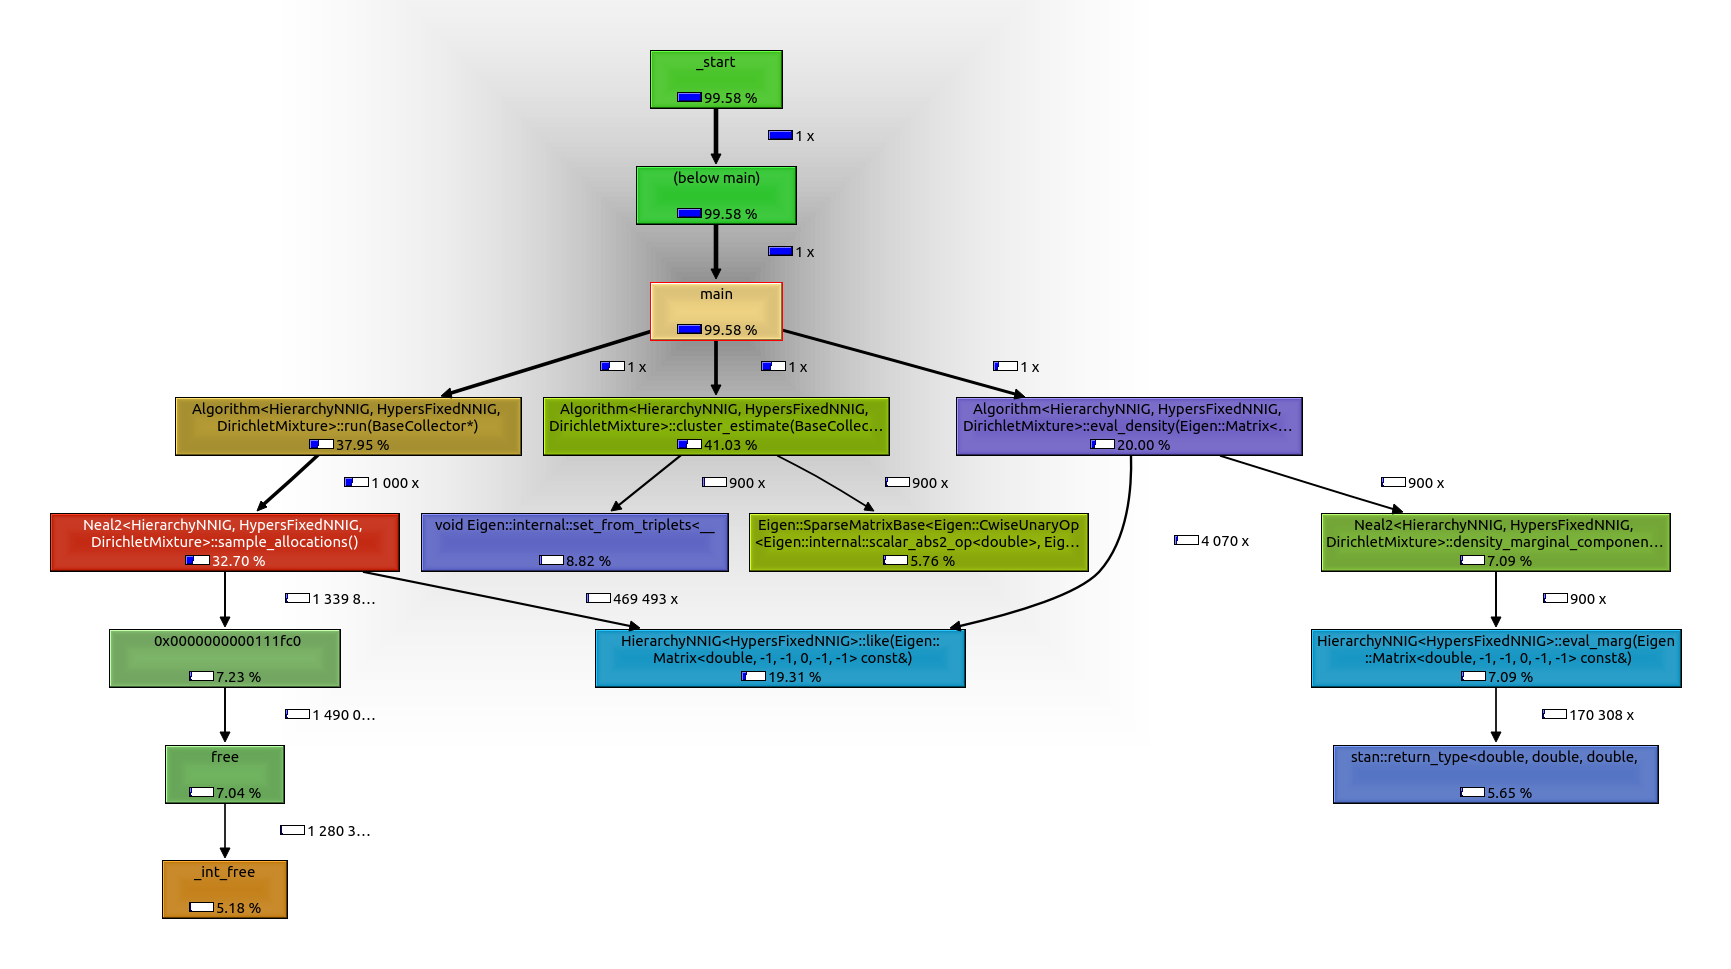
\includegraphics[scale=0.35]{etc/kcg_uni.png}
	%\captionsetup{labelformat=empty}
	\caption{\texttt{callgrind} dependence graph for \texttt{maintest\_uni.cpp} (univariate NNIG case).}
	\label{fig:profiling_nnig}
\end{figure}
The output of the univariate case produced the above dependence graph (figure \ref{fig:profiling_nnig}).
The percentage inside the square is the proportion of the total time spent in that particular function across all calls to it.
The number followed by x tells instead the number of times that function was called. \\
We are first interested in the partitioning of the computation time between the different methods.
We note that \verb|run()| has slightly less than 40\% of the total time, while \verb|eval_density()| has around 20\%, and \verb|cluster_estimate()| slightly more than 40\%.
As for the lower-level operations in \verb|run()|, almost all the time is spent in \verb|step()|, more specifically in \verb|sample_allocations()| (33\%).
This also means that the cost of collecting the states into the \verb|MemoryCollector| is irrelevant.
Moreover, \verb|like()| is the most significant low-level utility function in the library, taking a total of 20\% of the total time across both \verb|run()| and \verb|eval_density()|. \\

Let us now compare these results with the multivariate case, as shown in figure \ref{fig:profiling_nnw} in the next page.
As for the general composition, \verb|run()| has now become less than 10\% of the total, with \verb|sample_allocations()| taking roughly half of that amount, while the \verb|eval_density()| part reaches almost 90\%.
This is to be expected since nearly all of the time is spent likelihood and marginal computation, which is much harder in 2D than in the univariate case due to the introduction of matrix algebra.
We can also note that as a side effect of the growth of the density estimation part, the percentage of time spent in \verb|cluster_estimate()| is now irrelevant, which makes sense since the computational costs of building a dissimilarity matrix is almost identical in all dimensions.
The most costly part of the density estimation is the unoptimized \verb|eval_marg()| (more than 60\%), presumably due to the presence of matrix inversions and Student's $t$ evaluations, both of which require expensive Cholesky decompositions.
\begin{figure}[h]
	\hspace{-60pt}
	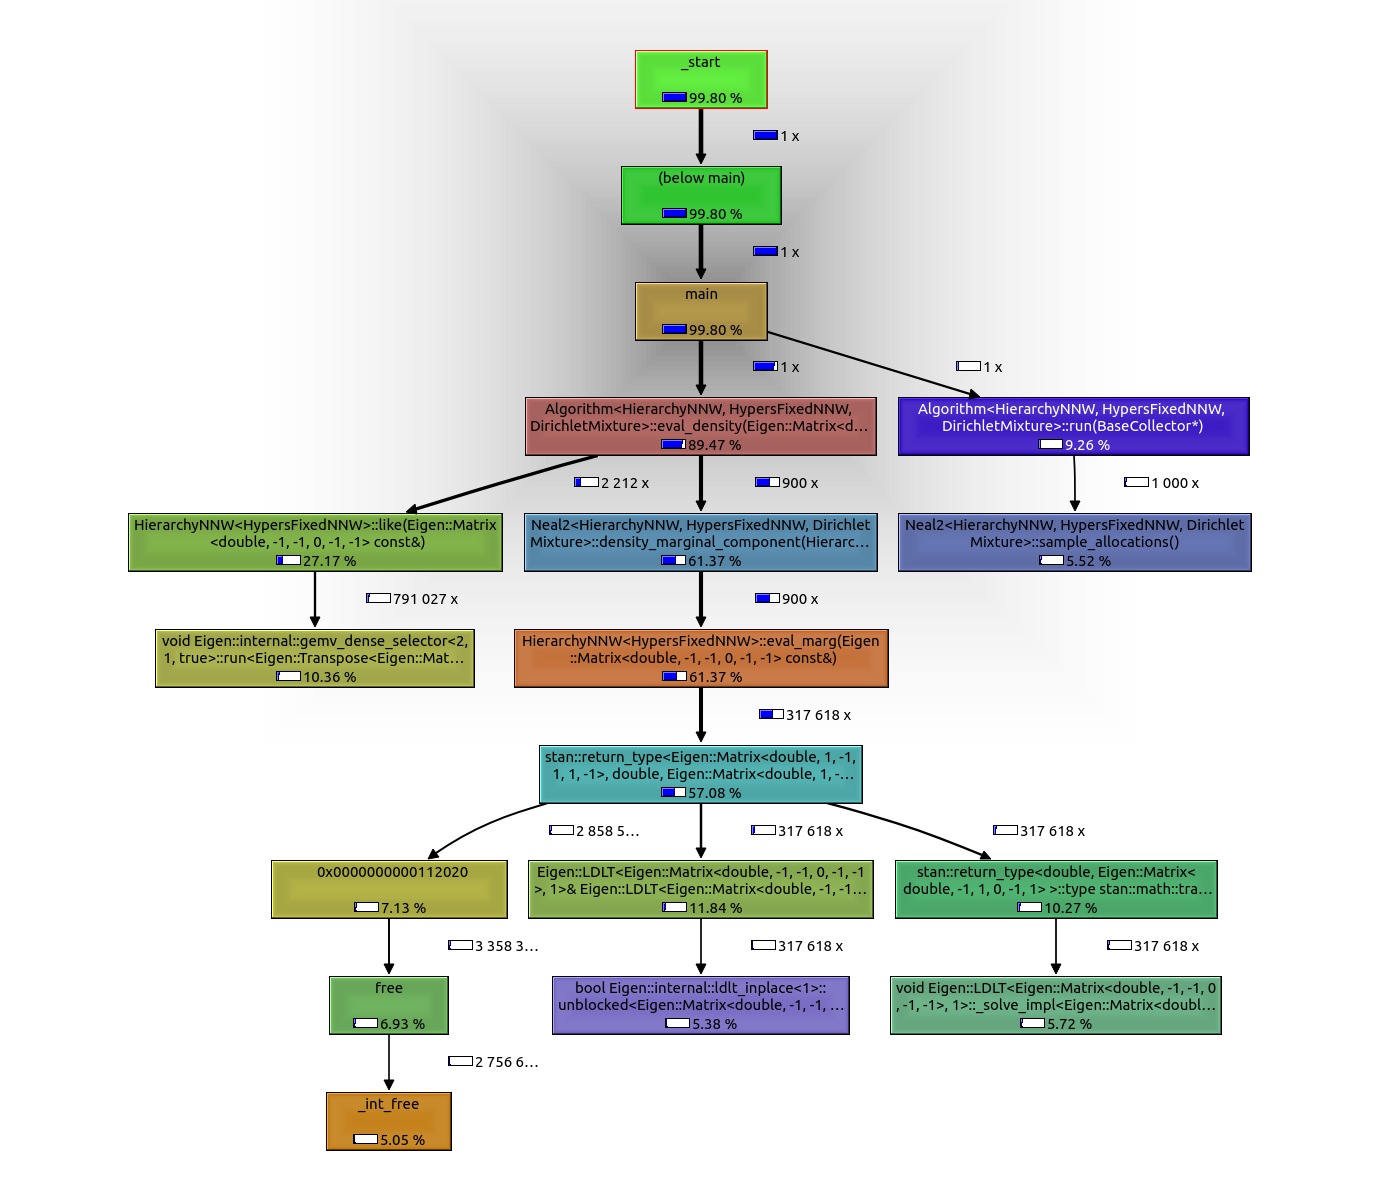
\includegraphics[scale=0.45]{etc/kcg_multi.png}
	%\captionsetup{labelformat=empty}
	\caption{\texttt{callgrind} dependence graph for \texttt{maintest\_multi.cpp} (multivariate NNW case).}
	\label{fig:profiling_nnw}
\end{figure}
On the contrary, we note that the usage of \verb|like()| is in the same order of magnitude as before (27\%).
Since the estimate algorithm is the same as before, this means that \verb|like()| is optimized enough for it to withstand the jump to the multidimensional case better than the other functions. \\
As for a final comparison with the case lacking the compiler flags described in section (\ref{opt-flags}), the optimization mainly impacts the multivariate case, with \verb|run()| being the main recipient, going from a whopping 58\% to the already mentioned 10\%.
In the univariate case, everything evenly benefits from the speedup, with the only relevant difference being for \verb|like()| which goes from over 30\% to 20\%.


\section{Limits}
Despite the optimizations in the \verb|cluster_estimate()| function, the storing of a number of large matrices still requires a considerable amount of memory.
In general, the Protobuf structures also become overwhelmingly large if the data dimension increases.
For these reasons, we were not able to run the multivariate Python tests (see chapter \ref{chap-py-test}) in higher dimensions such as $d=10$ and $d=20$ on our machines. \\
Another problem related to large dimensions arises when trying to run the \verb|Neal8| algorithm with 5-dimensional data.
At one point, the computed covariance matrix in one of the functions of the hierarchy becomes not symmetric.
Since a covariance/precision matrix must be symmetric and the Stan library implements a check for this property when passing such matrices as arguments to the density functions, the execution stops.
This error is likely due to the fact that the more the dimension of a space increases, the more its points will be far apart from each other -- this is the so-called ``curse of dimensionality''.
Since variance is a form of distance, the huge gap between points leads to a covariance matrix with large entries; due to the increased order of magnitude of these numbers, the floating-point approximations which are normally too small to appear become significant.
The hierarchy state is actually a precision matrix, which is the inverse of covariance and therefore should have very small values, but the computation of some covariance matrices is still required at some points.
